\chapter{Metodologia}
\label{chap:metodologia}

Este estudo utiliza dados previamente coletados de atletas profissionais de basquetebol feminino em repouso, abrangendo medidas de eletroencefalografia (EEG) e eletromiografia (EMG). O objetivo principal é investigar a sincronicidade entre sinais neurofisiológicos e musculares e avaliar como a estimulação transcraniana por corrente contínua de alta definição (HD-tDCS) catódica, aplicada sobre o córtex pré-frontal dorsolateral esquerdo, pode modular a atividade neural em condições de repouso, fornecendo insights sobre potenciais efeitos neuromodulatórios em atletas

\section{Participantes e Coleta de Dados}

O estudo foi aprovado pelo Comitê de Ética em Pesquisa da UFABC (protocolo: 08070819.1.0000.5594) e conduzido em conformidade com os princípios éticos estabelecidos pela Declaração de Helsinque para experimentos envolvendo seres humanos. Todas as participantes assinaram o Termo de Consentimento Livre e Esclarecido (TCLE) antes do início da coleta de dados.

Foram selecionadas atletas de elite, caracterizadas por:
\begin{itemize}
    \item Participação regular no programa de treinamento da equipe;
    \item Regime de treinamento superior a 10 horas semanais;
    \item Ausência de doenças ou lesões que pudessem interferir na execução do protocolo.
\end{itemize}

A amostra foi detalhadamente caracterizada por meio da mensuração de parâmetros como massa corporal e estatura, além da coleta de informações pessoais e esportivas (nome, data de nascimento, categoria, experiência esportiva, posição no time, fase da temporada, membro dominante e estilo de arremesso). Devido a problemas técnicos durante a coleta, apenas os dados de 6 atletas foram incluídos nas análises. Embora o número reduzido de participantes represente uma limitação, essa característica é comum em estudos com populações de difícil acesso, como atletas de elite. Estudos prévios, como o de Boukrina et al. \cite{boukrina2020considerations}, ressaltam que, em tais situações, estratégias de homogeneidade da amostra e análises que levem em conta a variabilidade individual podem produzir resultados robustos e significativos.

\section{Delineamento Experimental}

O estudo adotou um delineamento experimental randomizado, cruzado e duplo-cego, amplamente utilizado em pesquisas de neurociência aplicada e psicofisiologia para minimizar vieses e assegurar a validade dos resultados. Esse modelo permitiu que cada participante fosse submetida, em momentos distintos, tanto à condição ativa catódica de estimulação catódica (HD-tDCS) quanto à condição sham, fortalecendo as comparações intraindividuais.

Antes do início das sessões experimentais, foi realizada uma sessão de familiarização na qual as atletas receberam informações detalhadas sobre os objetivos, procedimentos, riscos e benefícios do estudo, além de treinamento prático para se familiarizarem com o protocolo e os equipamentos utilizados.

\begin{figure}[htb]
    \centering
    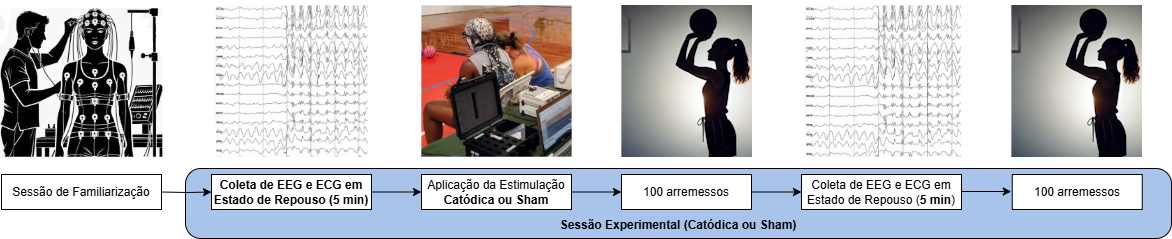
\includegraphics[width=0.9\textwidth]{figs/0_intro_e_desenho_experimental/desenho_experimental_drawio.png}
    \caption{Fluxo do protocolo experimental, incluindo a sessão de familiarização, as duas sessões experimentais (com estimulação catódica ou sham), as coletas de EEG/ECG em repouso e a execução de 200 arremessos por sessão.}
    \label{fig:desenho_experimental}
\end{figure}

As sessões experimentais seguiram a seguinte estrutura:
\begin{itemize}
    \item \textbf{Sessão 1:} Familiarização com os dispositivos e procedimentos do estudo.
    \item \textbf{Sessões 2 e 3:} Execução do protocolo experimental, no qual cada atleta realizou 200 arremessos por sessão, totalizando 400 arremessos.
\end{itemize}

Para garantir a padronização das condições ambientais, todas as sessões foram realizadas no mesmo local e horário do treinamento habitual das atletas. A ordem de aplicação das condições (HD-tDCS ativa e sham) foi definida aleatoriamente para cada participante, conforme o modelo cruzado.

\section{Questionários e Escalas}

Durante a coleta dos dados experimentais, foram aplicados questionários e escalas com o intuito de avaliar aspectos subjetivos relacionados ao estado psicológico e fisiológico das atletas. Embora esses instrumentos tenham sido incluídos no protocolo inicial com a finalidade de fornecer uma visão complementar às medidas neurofisiológicas, os dados obtidos não foram utilizados nas análises estatísticas ou nos resultados apresentados neste estudo. Os instrumentos aplicados foram:

\begin{itemize} \item \textbf{Escala de Qualidade Total de Recuperação (TQR):} Avalia a percepção subjetiva do estado geral de recuperação física e mental após as sessões experimentais. \item \textbf{Escala de Percepção Subjetiva de Esforço (PSE):} Mensura o esforço percebido pelas participantes durante as sessões experimentais. \item \textbf{Sport Competition Anxiety Test (SCAT):} Identifica níveis de ansiedade competitiva das participantes. \item \textbf{Questionário de Motivação Relacionado ao Exercício:} Investiga os fatores motivacionais das participantes durante o período experimental. \end{itemize}

Dessa forma, apesar de terem sido coletados, os dados desses questionários não são apresentados nem discutidos, dado o escopo específico das análises neurofisiológicas deste trabalho.

\section{Estimulação Transcraniana por Corrente Contínua de Alta Definição (HD-tDCS)}

A HD-tDCS foi realizada com um estimulador digital MxN da Soterix Medical, utilizando eletrodos de Ag/AgCl posicionados em uma touca de EEG. O posicionamento dos eletrodos seguiu um protocolo padronizado baseado em modelagem computacional, garantindo precisão e focalidade na estimulação \cite{datta2008transcranial}. Foram aplicadas duas condições experimentais: estimulação catódica (ativa) e sham (simulada), com as participantes expostas a ambas em sessões diferentes, de forma cruzada e randomizada. A calibração dos equipamentos foi realizada antes de cada sessão para assegurar a qualidade e a confiabilidade dos dados registrados.

\subsection{Processamento e Análise de Dados}

O processamento e a análise dos dados seguiram um fluxo estruturado que abrange desde a coleta e organização dos arquivos até a extração das métricas de sincronização e a aplicação de testes estatísticos para avaliar as diferenças entre as condições experimentais. A Figura~\ref{fig:fluxo_processamento} apresenta um diagrama geral dessas etapas.

\begin{figure}[htb]
    \centering
    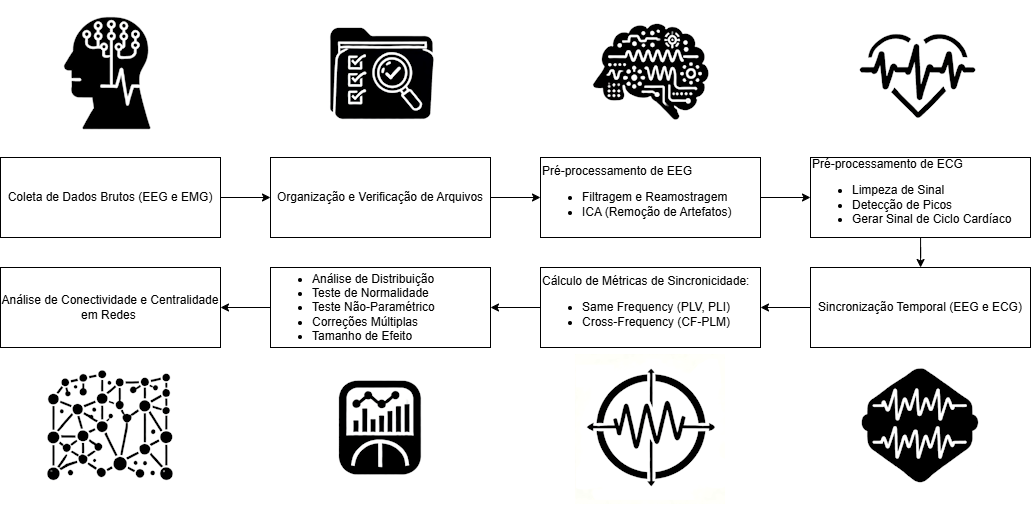
\includegraphics[width=0.9\textwidth]{figs/0_intro_e_desenho_experimental/diagrama_processamento_e_analise_drawio.png}
    \caption{Fluxo geral de processamento e análise de dados, desde a coleta e organização dos arquivos, passando pelas etapas de pré-processamento (EEG e ECG), sincronização temporal, extração de métricas de sincronização (PLI, PLV e CF-PLM) e, por fim, análises estatísticas e de conectividade em rede.}
    \label{fig:fluxo_processamento}
\end{figure}

\subsubsection{Pré-processamento de Dados}
Os sinais de EEG e EMG foram submetidos a etapas de pré-processamento que incluíram a filtragem de ruídos e a remoção de artefatos por meio de Independent Component Analysis (ICA). Paralelamente, os sinais de ECG passaram por processos de detecção de picos e extração do ciclo cardíaco, garantindo assim a qualidade e a consistência dos dados analisados.

\subsubsection{Sincronização de Sinais}
Para possibilitar uma análise integrada, os sinais de EEG e ECG foram alinhados temporalmente, assegurando que as medidas extraídas estivessem sincronizadas e pudessem ser comparadas corretamente.

\subsubsection{Cálculo de Sincronização Funcional}
A sincronização entre os sinais foi avaliada utilizando três métricas. O Phase Locking Value (PLV) e o Phase Lag Index (PLI) foram aplicados para quantificar a conectividade na mesma faixa de frequência, enquanto a Cross-Frequency Phase Linearity Measurement (CF-PLM) foi empregada para avaliar o acoplamento entre frequências distintas. Antes de sua aplicação nos dados experimentais, esses métodos foram testados e validados utilizando sinais simulados.

\subsubsection{Análise Estatística} Para investigar as diferenças entre as condições experimentais, aplicamos métodos estatísticos robustos, incluindo testes de normalidade, testes não paramétricos e correções para comparações múltiplas. Adicionalmente, foram utilizadas medidas de centralidade em redes para avaliar a conectividade funcional entre diferentes regiões corticais. Os padrões de conectividade foram representados por meio de gráficos e redes, facilitando a visualização e a interpretação dos resultados.

Esse fluxo sistemático permitiu uma abordagem rigorosa para explorar a sincronicidade cerebral e avaliar o impacto da estimulação transcraniana na conectividade neural das atletas em estado de repouso.
